\ifdefined\handout
  \documentclass[handout]{beamer}
\else
  \documentclass{beamer}
\fi

\usetheme{boxes}
\usecolortheme{structure}

\setbeamertemplate{footline}[frame number]

\ifdefined\handout
\definecolor{beamer@structure@color}{rgb}{0,0,0}
\setbeamertemplate{navigation symbols}{}
\setbeamercolor{normal text}{fg=black,bg=white}
\setbeamertemplate{frametitle}{\vskip 15pt\color{black}
\def\myhrulefill{\leavevmode\leaders\hrule height 1pt\hfill\kern 0pt}
\headingfont\insertframetitle\par\vskip-8pt\myhrulefill}
\else
\definecolor{beamer@structure@color}{rgb}{1,1,1}
\setbeamertemplate{navigation symbols}{}
\setbeamercolor{normal text}{fg=white,bg=black}
\setbeamertemplate{frametitle}{\vskip 15pt\color{white}
\def\myhrulefill{\leavevmode\leaders\hrule height 1pt\hfill\kern 0pt}
\headingfont\insertframetitle\par\vskip-8pt\myhrulefill}
\fi

\usepackage{amsmath,amssymb}

\newcommand{\NN}{\mathbb{N}}
\newcommand{\ZZ}{\mathbb{Z}}

\DeclareMathOperator{\mcd}{mcd}
\DeclareMathOperator{\mcm}{mcm}

\usepackage[spanish]{babel}

\usepackage{tikz-cd}
\usetikzlibrary{babel}
\usetikzlibrary{calc}

\usepackage{framed}

\newcommand{\dfn}{\mathrel{\mathop:}=}
\newcommand{\rdfn}{=\mathrel{\mathop:}}

\usepackage{mathspec}
\setsansfont[BoldFont={IBM Plex Sans Bold}, ItalicFont={IBM Plex Sans Italic}]{IBM Plex Sans}
\setmonofont[BoldFont={IBM Plex Mono Bold}, ItalicFont={IBM Plex Mono Italic}]{IBM Plex Mono}
\setmathrm[BoldFont={IBM Plex Sans Bold}, ItalicFont={IBM Plex Sans Italic}]{IBM Plex Sans}
\newfontfamily\headingfont[]{IBM Plex Sans Bold}

\setbeamercovered{transparent=10}


\usepackage{cancel}

\begin{document}

\begin{frame}[plain,noframenumbering]
  \textbf{INTRODUCCIÓN A LA TEORÍA DE NÚMEROS}

  Alexey Beshenov $\mid$ \texttt{cadadr.org}

  \vfill

  \begin{center}\huge\headingfont
    TEOREMA FUNDAMENTAL

    DE LA ARITMÉTICA
  \end{center}

  \vfill
\end{frame}

\begin{frame}[plain,noframenumbering]

  \vfill

  \begin{center}\huge\headingfont
    UN POCO DE LA HISTORIA
  \end{center}

  \vfill
\end{frame}

\begin{frame}
  \frametitle{EUCLIDES, «ELEMENTOS» (ca. 300 a.C.)}

  \begin{itemize}
  \item<2-> \textbf{Libro VII, Proposición 30}. «Si dos números, al
    multiplicarse entre sí, hacen algún número y algún número primo mide a su
    producto, también medirá a uno de los números iniciales».

    («Lema de Euclides»: $p \mid ab \Longrightarrow p\mid a\text{ o } p\mid b$.)

  \item<3-> \textbf{Libro VII, Proposición 31}. «Todo número compuesto es medido
    por algún número primo».

    \textbf{Proposición 32}. «Todo número o bien es número primo o es medido por
    algún número primo».
 
    ($n > 1 \Longrightarrow p \mid n$ para algún primo.)

  \item<4-> \textbf{Libro IX, Proposición 14}. «Si un número es el menor medido
    por números primos, no será medido por ningún otro número primo fuera de los
    que le medían desde un principio».

    ($\mcm (p_1,\ldots,p_s)$ no es divisible por primo $q \ne p_1,\ldots,p_s$.)
  \end{itemize}
\end{frame}

\begin{frame}
  \frametitle{TABLAS DE FACTORIZACIÓN}

  \onslide<2->{Johann Rahn, 1659, tabla de divisores más pequeños $p \mid n$
    para $n < 24\,000$, donde $2, 5 \nmid n$.}
  % https://books.google.com/books?id=ZJg_AAAAcAAJ

  \visible<3->{\begin{center}
      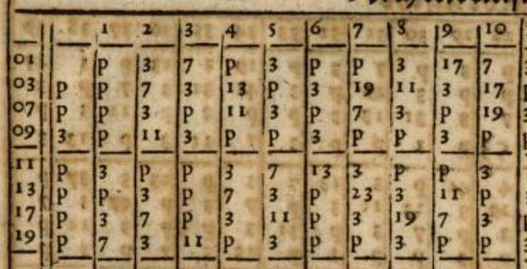
\includegraphics[width=0.6\textwidth]{pic/rahn.jpg}
    \end{center}}

  \onslide<4->{Ejemplo: $611 = 13\cdot 47$ y $613$ es primo.}
\end{frame}

\begin{frame}
  \frametitle{TABLAS DE FACTORIZACIÓN}

  \onslide<2->{Johann Poetius, 1728, tabla de factorizaciones completas para
    $n < 10\,000$ («anatomia numerorum», \emph{anatomía de los números}).}
  % https://www.digitale-sammlungen.de/en/view/bsb10082579
 
  \visible<3->{\begin{center}
      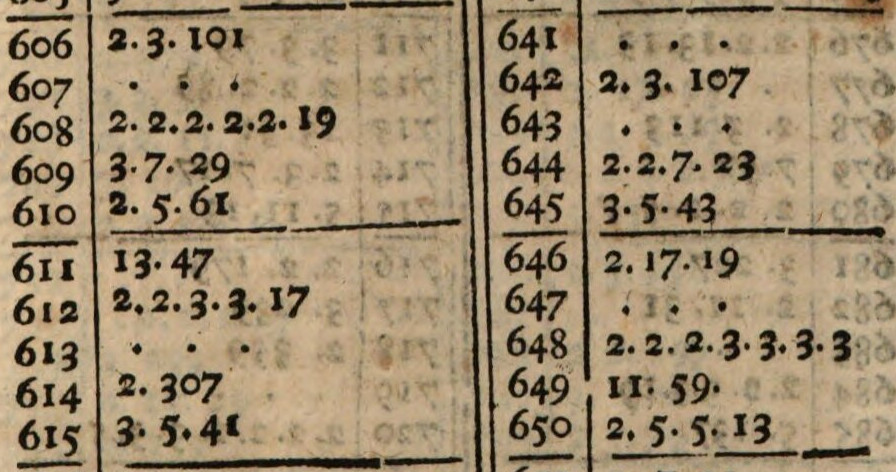
\includegraphics[width=0.8\textwidth]{pic/poetius.jpg}
    \end{center}}
\end{frame}

\begin{frame}
  \frametitle{ENUNCIADOS SIN LA UNICIDAD}

  \onslide<2->{La posibilidad de descomponer todo número en un producto de
      primos se menciona en varios textos del siglo XVIII.}

  \begin{itemize}
  \item<3-> Euler «Vollständige Anleitung zur Algebra» (1770)

    (\emph{Guía completa de álgebra}), Cap. IV, no. 41.

  \item<4-> Legendre, «Essai sur la théorie des nombres» (1798)

    (\emph{Ensayo sobre la teoría de números}), Introduction, \S VIII.
  \end{itemize}
\end{frame}

\begin{frame}
  \frametitle{GAUSS, «DISQUISITIONES» (1801)}

  \onslide<2->{«Disquisitiones arithmeticae», Sectio secunda, no. 16:

    \vspace{1em}

    «Numerus compositus quicunque \underline{unico tantum modo} in factores
    primos resolui potest».

    \vspace{1em}

    (Cualquier número compuesto puede resolverse en factores primos
    \underline{de modo único}.)}
\end{frame}

\begin{frame}[plain,noframenumbering]

  \vfill

  \begin{center}\huge\headingfont
    DEMOSTRACIÓN
  \end{center}

  \vfill
\end{frame}

\begin{frame}
  \frametitle{FACTORIZACIÓN EN PRIMOS}

  \begin{itemize}
  \item<2-> $p > 1$ es \textbf{primo} si
    $d \mid p \Longrightarrow d = \pm 1, \pm p$.

  \item<3-> Para dos primos $p \mid q \Longrightarrow p = q$.

  \item<4-> \textbf{Lema de Euclides}:
    $p \mid ab \Longrightarrow p\mid a \text{ o }p\mid b$.

  \item<5-> Todo $n > 1$ tiene un divisor primo:
    \begin{gather*}
      p = d_i \mid d_{i-1} \mid \cdots \mid d_1 \mid d_0 = n, \\
      d_i < d_{i-1} < \cdots < d_1 < d_0.
    \end{gather*}

  \item<6-> Todo $n > 1$ se descompone en primos:
    $$p_1 \mid n, ~ p_2 \mid \frac{n}{p_1}, ~ p_3 \mid \frac{n}{p_1 p_2}, ~ p_4 \mid \frac{n}{p_1 p_2 p_3}, ~ \ldots, ~ n = p_1 \cdots p_s.$$
  \end{itemize}
\end{frame}

\begin{frame}
  \frametitle{TEOREMA FUNDAMENTAL DE LA ARITMÉTICA}

  \begin{itemize}
  \item<2-> Todo $n \ne 0$ puede ser escrito como
    $$n = \pm p_1 \cdots p_s,$$
    donde los $p_i$ son primos (no necesariamente distintos).

  \item[*]<3-> Si $n = \pm 1$, entonces $s = 0$ (producto vacío).

  \item<4-> Para dos factorizaciones de esta forma
    $$\pm p_1 \cdots p_s = \pm q_1 \cdots q_t$$
    necesariamente $s = t$ y $p_i = q_i$ para $i = 1,\ldots,s$,
    después de una permutación de los índices.
  \end{itemize}
\end{frame}

\begin{frame}
  \frametitle{DEMOSTRACIÓN DE LA UNICIDAD}

  \onslide<2->{\[ p_1 \cdots p_s = q_1 \cdots q_t. \]}

  \begin{itemize}
  \item<3-> \textbf{Lema de Euclides}:
    $p_s \mid q_1 \cdots q_t \Longrightarrow p_s \mid q_i \Longrightarrow p_s = q_i$

    para algún $i = 1,\ldots,t$.

  \item<4-> Después de una renumeración, $i = t$.

  \item<5-> $p_1 \cdots p_{s-1} \cancel{p_s} = q_1 \cdots q_{t-1} \cancel{q_t}$.

  \item<6-> . . . . .

  \item<7-> Llegamos a la conclusión que $s = t$ y $p_i = q_i$ después de una
    permutación de los índices. \qed
  \end{itemize}
\end{frame}

\begin{frame}
  \frametitle{OTRA FORMULACIÓN}

  \begin{itemize}
  \item<2-> Todo entero $n \ne 0$ se escribe de modo único como
    $$n = \pm p_1^{e_1}\cdots p_s^{e_s},$$
    donde $p_1, \ldots, p_s$ son diferentes primos y $e_i \ge 0$.

  \item<3-> Todo número racional $x = \frac{a}{b} \ne 0$ se escribe de modo
    único como
    $$x = \pm p_1^{e_1}\cdots p_s^{e_s},$$
    donde $p_1, \ldots, p_s$ son diferentes primos y $e_i \in \ZZ$.

  \item<4-> La potencia $e_i$ de $p_i$ es la \textbf{valuación $p_i$-ádica} del
    número.

  \item<5-> En otra ocasión: valuaciones $p$-ádicas.
    \onslide<6->{\begin{gather*}
      v_2 (252) = 2, ~
      v_3 (252) = 2, ~
      v_7 (252) = 1, \\
      v_p (252) = 0 \text{ si } p\ne 2,3,7, \quad 257 = 2^2\cdot 3^2\cdot 7.
    \end{gather*}}
    \end{itemize}
\end{frame}

\begin{frame}
  \frametitle{ALGORITMOS}

  \begin{itemize}
  \item<2-> Existen algoritmos rápidos que verifican si $p$ es primo.

    \textbf{Algoritmo probabilista de Miller--Rabin} (1980).

    \textbf{Algoritmo determinista AKS} (Agrawal--Kayal--Saxena, 2002).

  \item<3-> No se conocen (probablemente no existen) algoritmos rápidos de
    factorización en primos. Esta es la base de la
    \textbf{criptografía de clave pública}.

  \item<4-> El mejor algoritmo práctico para grandes números:

    la \textbf{criba del cuerpo de números}
    (Pollard--Lenstra--Lenstra--\dots, 1988).

  \item<5-> El \textbf{algoritmo de Shor} (1994) para las computadoras
    cuánticas. Todavía tiene poco valor práctico.
  \end{itemize}
\end{frame}

\begin{frame}[plain,noframenumbering]

  \vfill

  \begin{center}\huge\headingfont
    ALGUNAS APLICACIONES

    (EJERCICIOS)
  \end{center}

  \vfill
\end{frame}

\begin{frame}
  \frametitle{EJERCICIO 1: REINTERPRETACIÓN\\DEL MCD Y MCM}

  \onslide<2->{\begin{framed}
      Escribamos
      \[
        m = p_1^{e_1}\cdots p_s^{e_s},
        \quad
        n = p_1^{e'_1}\cdots p_s^{e'_s},
      \]
      donde $p_i$ son primos y $e_i, e_i' \ge 0$. Luego,
      \[ m \mid n \iff e_i \le e'_i \text{ para todo }i. \]
      \[
        \mcd (m,n) = \prod_i p_i^{\min \{ e_i, e_i' \}},
        \quad
        \mcm (m,n) = \prod_i p_i^{\max \{ e_i, e_i' \}}.
      \]
    \end{framed}}

  \onslide<3->{\textbf{Demostración}. Ejercicio.}
\end{frame}

\begin{frame}
  \frametitle{REINTERPRETACIÓN DEL MCD Y MCM (CONTINUACIÓN)}

  \begin{itemize}
  \item<2-> \textbf{Ejemplo}:
    \begin{align*}
      \mcd (120, 90) & = \mcd (2^3\cdot 3\cdot 5, \, 2\cdot 3^2\cdot 5) = 30, \\
      \mcm (120, 90) & = 2^3\cdot 3^2\cdot 5 = 360.
    \end{align*}

  \item<3-> mcd y mcm se calculan con el algoritmo de Euclides que es muy
    rápido, mientras que la factorización es difícil.

  \item<4-> Nuestra prueba del teorema fundamental usa el mcd:

    $\text{existencia del mcd} \Longrightarrow
    \text{lema de Euclides} \Longrightarrow
    \text{teorema fundamental}$.
  \end{itemize}
\end{frame}

\begin{frame}
  \frametitle{EJERCICIO 2: DIVISIBILIDAD POR NÚMEROS COPRIMOS}

  \begin{itemize}
  \item<2-> Demuestre que si $\mcd (a,b) = 1$, entonces
    $$a \mid c, \, b \mid c \Longrightarrow ab \mid c.$$

  \item<3-> Demuestre que para todo $n$ se tiene
    \[
      30 \mid (n^5 - n),
      \quad
      42 \mid (n^7 - n).
    \]

    \onslide<4->{Ejemplo:
    \begin{align*}
      2^2 - 2 & = 30,\\
      3^2 - 3 & = 240 = 30\cdot 8,\\
      4^2 - 4 & = 1020 = 30\cdot 34,\\
      5^2 - 5 & = 3120 = 30\cdot 104,\\
              & \cdots
    \end{align*}}
  \end{itemize}
\end{frame}

\begin{frame}
  \frametitle{EJERCICIO 3: N-ÉSIMAS POTENCIAS}

  \begin{itemize}
  \item<2-> Demuestre que $n = p_1^{e_1}\cdots p_s^{e_s}$ es un cuadrado
    ($n = m^2$ para algún $m$) si y solamente si los $e_i$'s son pares.

  \item<3-> Demuestre que si $a^2 = bc$ y $\mcd (b,c) = 1$, entonces
    $b = b'^2$ y $c = c'^2$ para algunos $b', c' \in \ZZ$.

  \item<4-> Generalice estas observaciones a $n$-ésimas potencias.
  \end{itemize}
\end{frame}

\begin{frame}
  \frametitle{EJERCICIO 4: FUNCIÓN DE MÖBIUS μ}

  \begin{itemize}
  \item<2-> Si $p^2 \mid n$ para algún $p$, entonces $\mu (n) \dfn 0$.

  \item<3-> Si $n = p_1\cdots p_s$ para diferentes primos $p_i$, entonces
    $\mu (p_1\cdots p_s) \dfn (-1)^s$.

  \item<4-> Demuestre que
    $\sum_{d\mid n} \mu (d) = 0$,
    donde la suma es sobre los divisores positivos de $n$.

    \onslide<5->{Ejemplo:
    \begin{multline*}
      \mu(1) + \mu(2) + \mu(3) + \mu(4) + \mu(6) + \mu(9) + \mu(12) + \mu(18) + \mu(36) \\
      = 1 - 1 - 1 + 0 + 1 + 0 + 0 + 0 + 0 = 0.
    \end{multline*}}

  \item<6-> En otra ocasión: \textbf{inversión de Möbius}.
  \end{itemize}
\end{frame}

\begin{frame}[plain,noframenumbering]

  \vfill

  \begin{center}\huge\headingfont
    ¡GRACIAS POR SU ATENCIÓN!
  \end{center}

  \vfill
\end{frame}
\end{document}
